\section{Auswertung}
\label{sec:Auswertung}
Der Versuch wird, wie in \autoref{sec:Durchführung} aufgebaut und durchgeführt.
\subsection{Bestimmung der Weglänge}
\label{subsec:Weglänge}
Im Folgenden wird die mittlere Weglänge bei verschiedenen Temperaturen bestimmt. Dazu wird mit \autoref{eqn:psät} der Sättigungsdampfdruck $p_{sät}$ bei den gemessenen 
Temperaturen bestimmt. Danach wird $\bar{\omega}$ mit der \autoref{eqn:Weglänge} bestimmt. Alle Werte werden in die \autoref{tab:Weglänge} eingetragen.
\begin{table}[H]
  \centering
  \caption{Gemsesene und bestimmte Werte für die Wellenlänge.}
  \label{tab:Wellenlänge}
  \sisetup{table-format=2.2}
  \begin{tabular}{S[table-format=2.0] S[table-format=1.0] S[table-format=4.0] }
  \toprule
  {Temperaturen $T / \si{\kelvin}$} & {Sättigungsdampfdruck $p_{sät} / \si{\milli\bar}$} & {mittlere Weglänge $\bar{\omega} / \si{\centi\meter}}$}\\
  \midrule
     5   & 5 & 2440  \\
    10  & 5 & 2440  \\
    14  & 4 & 3050  \\
    19  & 5 & 2440  \\
  \bottomrule
  \end{tabular}
\end{table}

%Ende der Weglänge

\subsection{Integrale und differentielle Energieverteilung}
\label{subsec:Energieverteilung}



%Ende der Energieverteilung

\subsection{Franck-Hertz-Kurve} % (fold)
\label{sub:Franck-Hertz-Kurve}



% subsection Franck-Hertz-Kurve (end)

\begin{figure}
  \centering
  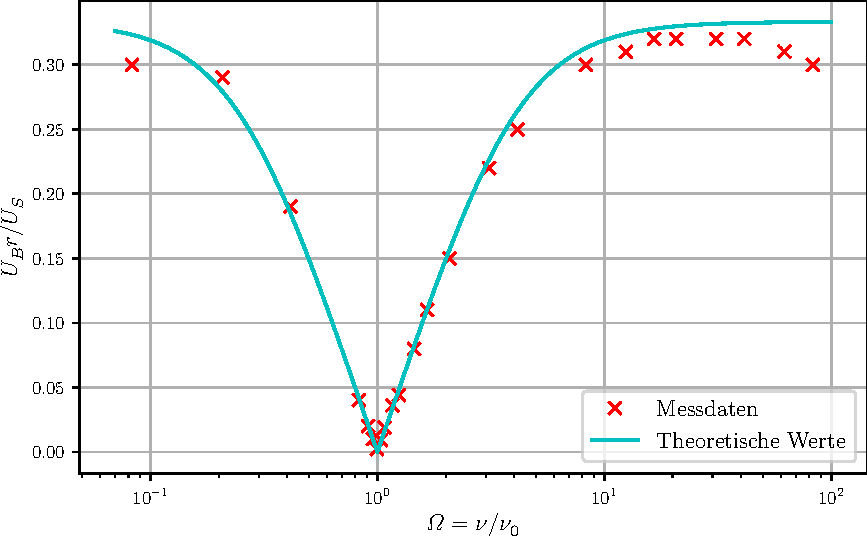
\includegraphics{plot.pdf}
  \caption{Plot.}
  \label{fig:plot}
\end{figure}



